\chapter{Requirement Analysis}
\label{chap:requirements}

\begin{chapterintro}
This chapter describes one of the most important stages in software development: the requirement analysis using different scenarios. For this, a detailed analysis of the possible use cases is made using the Unified Modeling Language (UML). This language allows us to specify, build and document a system using graphic language. 
\end{chapterintro}


\cleardoublepage

\section{Overview}
The result of this chapter will be a complete specification of the requirements, which will be matched by each module in the design stage. This helps us also to focus on key aspects and take apart other less important functionalities that could be implemented in future works.

%As commented before, our project aims to develop a personal assistance system that integrates the advantages of agent systems, information retrieval and Natural Language Processing. Our personal assistant should have the capability to solve user's questions using all of these features.

\section{Use cases}

These sections identify the use cases of the system. This helps us to obtain a complete specification of the uses of the system, and therefore define the complete list of requisites to match.  First, we will present a list of the actors in the system and a UML diagram representing all the actors participating in the different use cases. This representation allows, apart from specifying the actors that interact in the system, the relationships between them.

These use cases will be described the next sections, including each one a table with their complete specification. Using these tables, we will be able to define the requirements to be established.


\subsection{Actors dictionary}

\noindent The list of primary and secondary actors is presented in table \ref{tab:actores}. These actors participate in the different use cases, which are presented later.\\



\begin{table}[!htpb]
\centering
\begin{tabular}{|c|c|x{6cm}|}
\noalign{\hrule height 2pt}
\textbf{Actor identifier} & \textbf{Role} & \textbf{Description}\tn
\hline
ACT-1 & User & End user that uses Omelette mash-up Editor  to find a mash-up based on her goals, which are expressed using keywords\tn
\hline
ACT-2 & Developer & Technical developer which uses the OMR.\tn
\hline
ACT-4 & Admin & Administrator of the OMR, in charge of tasks such as inserting, deleting mash-ups, as well as including new available mash-up repositories..\tn
\hline
ACT-5 & MDP & mash-up Delivery Platform, component of the "Live Omelette Environment" that executes mash-ups..\tn
\hline
ACT-6 & External service & External services for executing actions.\tn
\noalign{\hrule height 2pt}
\end{tabular}
\caption{Actors list}
\label{tab:actores}
\end{table}




~\\



\FloatBarrier


\subsection{OMR composition and search use case}
This use case package collects the search functionalities of OMR, as shown in \ref{fig:pack-uc1}.

The use cases presented in this section are as shown in the Figure \ref{fig:pack-uc1}:
\begin{itemize}
\item \textit{keyword search} detailed in sub-section \ref{subsec:keywordsearch}.
\item \textit{mashup browse by category} detailed in sub-section \ref{subsec:mashupbrowsebycat}.
\item \textit{ask question}  detailed in sub-section \ref{subsec:askquestion}.
\item \textit{mashup search by query}  detailed in sub-section \ref{subsec:mashupsearchbyquery}.
\item \textit{mashup compose}  detailed in sub-section \ref{subsec:mashupcompose}.
\end{itemize}


\begin{figure}[h]
\centering
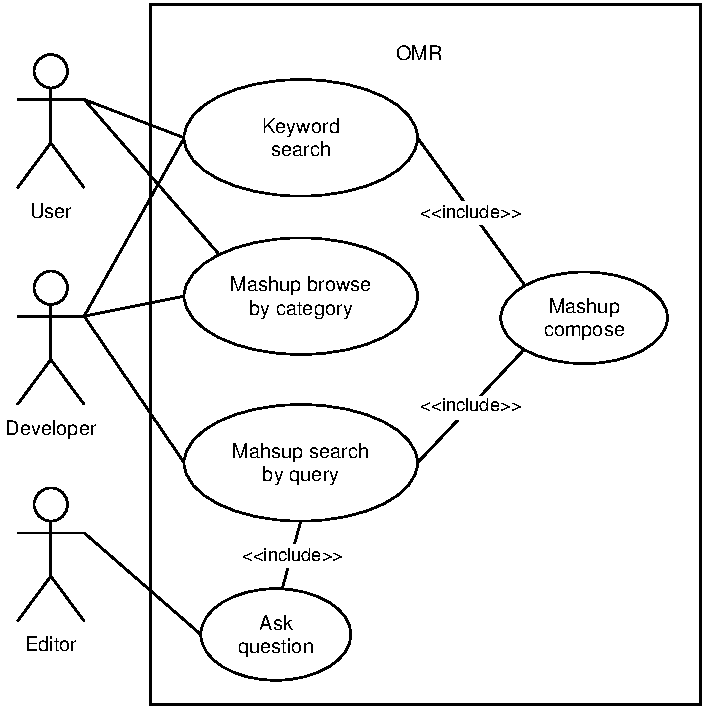
\includegraphics{graphics/uc1.pdf}
\caption{Composition and Search use case}
\label{fig:pack-uc1}
\end{figure}

\newpage
\subsubsection{Keyword search}
\label{subsec:keywordsearch}

\begin{table}[!htpb]
\centering
\begin{tabular}{|c|x{1cm}x{5cm}x{5cm}|}
\noalign{\hrule height 2pt}
\textbf{Use Case Name} & \multicolumn{3}{c|}{keyword search}\\
\hline
\textbf{Use Case ID} & \multicolumn{3}{x{11cm}|}{UC1.1}\\
\hline
\textbf{Pre-Condition} & \multicolumn{3}{x{11cm}|}{OMR  has been fed with  mash-ups and individual services}\\
\hline
\textbf{Post-Condition} & \multicolumn{3}{x{11cm}|}{Optionally, the developer completes the MDL definition to make a mash-up executable}\\
\hline
\textbf{Flow of Events} & \multicolumn{1}{c|}{} & \multicolumn{1}{x{5cm}|}{Actor Input} & \multicolumn{1}{x{5cm}|}{System Response}\\
\hline

\textbf{} & \multicolumn{1}{x{0.5cm}|}{1} & \multicolumn{1}{x{5cm}|}{The user / developer expresses her goals by using textual keywords} & \multicolumn{1}{x{5cm}|}{Ranked result list of mash-ups and individual services. The  mash-up can be an existing  mash-up or a new dynamically composed  mash-up, which can be executable or not. In the same way, the service can be automatically available in the editor or could require human intervention. }\\
\hline

\textbf{} & \multicolumn{1}{x{0.5cm}|}{2a} & \multicolumn{1}{x{5cm}|}{The user / developer access  service / mash-up metadata and   selects one  service / mash-up in order to use it} & \multicolumn{1}{x{5cm}|}{System shows details of the metadata service / mash-up.}\\
\hline

\textbf{} & \multicolumn{1}{x{0.5cm}|}{2b} & \multicolumn{1}{x{5cm}|}{The developer has obtained a non executable  mash-up and opens the editor to complete it} & \multicolumn{1}{x{5cm}|}{The system opens the mash-up editor, which allows the user to finish the mash-up composition (giving API details, etc.), completing the MDL, and finally, publishing the resulting  mash-up in the OMR.}\\
\hline


\end{tabular}
\end{table}

\FloatBarrier


\subsubsection{Mash-up browse by category}
\label{subsec:mashupbrowsebycat}


\begin{table}[!htpb]
\centering
\begin{tabular}{|c|x{1cm}x{5cm}x{5cm}|}
\noalign{\hrule height 2pt}
\textbf{Use Case Name} & \multicolumn{3}{c|}{mash-up browse by category}\\
\hline
\textbf{Use Case ID} & \multicolumn{3}{x{11cm}|}{UC1.2}\\
\hline
\textbf{Primary Actor} & \multicolumn{3}{c|}{User, Developer }\\
\hline
\textbf{Pre-Condition} & \multicolumn{3}{x{11cm}|}{OMR  has been fed with mash-ups and services and has categorized the service / mash-ups according to one or more categories. For example, users can follow a taxonomy based on their needs and types of applications, such as Appstore, while developers can follow a taxonomy based on the technology, integration needs, etc. }\\
\hline
\textbf{Post-Condition} & \multicolumn{3}{x{11cm}|}{-}\\
\hline
\textbf{Flow of Events} & \multicolumn{1}{c|}{} & \multicolumn{1}{x{5cm}|}{Actor Input} & \multicolumn{1}{x{5cm}|}{System Response}\\
\hline

\textbf{} & \multicolumn{1}{x{0.5cm}|}{1} & 
\multicolumn{1}{x{5cm}|}{The user / Developer selects a category} & 
\multicolumn{1}{x{5cm}|}{Ranked list of service / mash-ups belonging to that category}\\
\hline

\textbf{} & \multicolumn{1}{x{0.5cm}|}{2} & 
\multicolumn{1}{x{5cm}|}{The user / developer refines the search with filtering options} & 
\multicolumn{1}{x{5cm}|}{Filtered result set based on filtering options}\\
\hline


\end{tabular}
\end{table}
\FloatBarrier

\newpage
\subsubsection{mash-up search by query}
\label{subsec:mashupsearchbyquery}


\begin{table}[!htpb]
\centering
\begin{tabular}{|c|x{1cm}x{5cm}x{5cm}|}
\noalign{\hrule height 2pt}
\textbf{Use Case Name} & \multicolumn{3}{c|}{mash-up search by query}\\
\hline
\textbf{Use Case ID} & \multicolumn{3}{x{11cm}|}{UC1.3}\\
\hline
\textbf{Primary Actor} & \multicolumn{3}{c|}{Developer}\\
\hline
\textbf{Pre-Condition} & \multicolumn{3}{x{11cm}|}{OMR has been fed with service / mash-ups}\\
\hline
\textbf{Post-Condition} & \multicolumn{3}{x{11cm}|}{-}\\
\hline
\textbf{Flow of Events} & \multicolumn{1}{c|}{} & \multicolumn{1}{x{5cm}|}{Actor Input} & \multicolumn{1}{x{5cm}|}{System Response}\\
\hline

\textbf{} & \multicolumn{1}{x{0.5cm}|}{1} & 
\multicolumn{1}{x{5cm}|}{The developer executes a query using a query language (for example, SPARQL)} & 
\multicolumn{1}{x{5cm}|}{Result set of matching service / mash-ups}\\
\hline


\end{tabular}
\end{table}
\FloatBarrier

\newpage
\subsubsection{mash-up compose}
\label{subsec:mashupcompose}

\begin{table}[!htpb]
\centering
\begin{tabular}{|c|x{1cm}x{5cm}x{5cm}|}
\noalign{\hrule height 2pt}
\textbf{Use Case Name} & \multicolumn{3}{c|}{mash-up compose}\\
\hline
\textbf{Use Case ID} & \multicolumn{3}{x{11cm}|}{UC1.4}\\
\hline
\textbf{Primary Actor} & \multicolumn{3}{c|}{User, developer}\\
\hline
\textbf{Pre-Condition} & \multicolumn{3}{x{11cm}|}{OMR has been fed with individual services and  mash-ups}\\
\hline
\textbf{Post-Condition} & \multicolumn{3}{x{11cm}|}{Optionally, the developer completes the MDL definition to make a mash-up executable}\\
\hline
\textbf{Flow of Events} & \multicolumn{1}{c|}{} & \multicolumn{1}{x{5cm}|}{Actor Input} & \multicolumn{1}{x{5cm}|}{System Response}\\
\hline

\textbf{} & \multicolumn{1}{x{0.5cm}|}{1} & 
\multicolumn{1}{x{5cm}|}{The User / Developer expresses her goals using textual keywords} & 
\multicolumn{1}{x{5cm}|}{Since there is no service mash-up that fulfills the user goals, the system analyses potential combinations of available mash-ups in OMR and provides a composed mash-up or a template of a potential composition}\\
\hline

\end{tabular}
\end{table}
\FloatBarrier

\newpage
\subsubsection{Ask suggestion}
\label{subsec:askquestion}

\begin{table}[!htpb]
\centering
\begin{tabular}{|c|x{1cm}x{5cm}x{5cm}|}
\noalign{\hrule height 2pt}
\textbf{Use Case Name} & \multicolumn{3}{c|}{Ask suggestion}\\
\hline
\textbf{Use Case ID} & \multicolumn{3}{x{11cm}|}{UC1.5}\\
\hline
\textbf{Primary Actor} & \multicolumn{3}{c|}{Editor}\\
\hline
\textbf{Pre-Condition} & \multicolumn{3}{x{11cm}|}{OMR has been fed with individual services and  mash-ups}\\
\hline
\textbf{Post-Condition} & \multicolumn{3}{x{11cm}|}{}\\
\hline
\textbf{Flow of Events} & \multicolumn{1}{c|}{} & \multicolumn{1}{x{5cm}|}{Actor Input} & \multicolumn{1}{x{5cm}|}{System Response}\\
\hline

\textbf{} & \multicolumn{1}{x{0.5cm}|}{1} & 
\multicolumn{1}{x{5cm}|}{The mash-up editor requests a list of available service /   mash-ups to suggest them to the user} & 
\multicolumn{1}{x{5cm}|}{Ranked result list of  service / mash-ups expressed in MDL. The  mash-up can be an existing  mash-up or a new dynamically composed mash-up, which can be executable or not}\\
\hline

\end{tabular}
\end{table}
\FloatBarrier

\newpage
\subsection{OMR discovery and administration use case}
This use case package collects the main administration use cases of the OMR, as shown in \ref{fig:pack-uc2}

\begin{itemize}
\item \textit{automated mash-up feeding} detailed in subsection \ref{subsec:automatedmashupfeeding}
\item \textit{manual mash-up feeding} detailed in subsection \ref{subsec:manualmashupmanagement}
\item \textit{form discovery and description} detailed in subsection \ref{subsec:formdiscoveryanddescription}
\item \textit{mash-up registry integration} detailed in subsection \ref{subsec:mashupregistryintegration}
\item \textit{mash-up registry API based integration} detailed in subsection \ref{subsec:apibasedintegration}
\item \textit{mash-up registry Scrappy based integration} detailed in subsection \ref{subsec:scrappybasedintegration}
\item \textit{manual mash-up management} detailed in subsection \ref{subsec:manualmashupmanagement}
\item \textit{browse pending} detailed in subsection \ref{subsec:pending}
\item \textit{validate service} detailed in subsection \ref{subsec:validate}
\item \textit{reject service} detailed in subsection \ref{subsec:reject}
\end{itemize}

\begin{figure}[h]
\centering
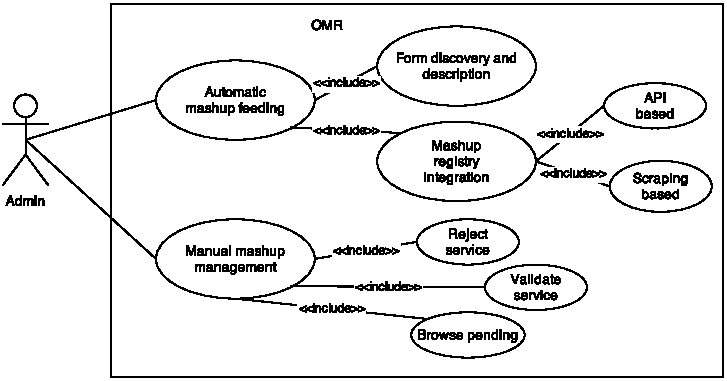
\includegraphics[width=400pt]{graphics/uc2.pdf}
\caption{OMR discovery and administration use case}
\label{fig:pack-uc2}
\end{figure}

\FloatBarrier

\newpage
\subsubsection{Automatic mash-up feeding}
\label{subsec:automatedmashupfeeding}

\begin{table}[!htpb]
\centering
\begin{tabular}{|c|x{1cm}x{5cm}x{5cm}|}
\noalign{\hrule height 2pt}
\textbf{Use Case Name} & \multicolumn{3}{c|}{Automatic mash-up feeding }\\
\hline
\textbf{Use Case ID} & \multicolumn{3}{x{11cm}|}{UC2.1}\\
\hline
\textbf{Primary Actor} & \multicolumn{3}{c|}{Admin}\\
\hline
\textbf{Pre-Condition} & \multicolumn{3}{x{11cm}|}{Availability of external service mash-up repositories or web sites}\\
\hline
\textbf{Post-Condition} & \multicolumn{3}{x{11cm}|}{Service / mash-ups are added to OMR}\\
\hline
\textbf{Flow of Events} & \multicolumn{1}{c|}{} & \multicolumn{1}{x{5cm}|}{Actor Input} & \multicolumn{1}{x{5cm}|}{System Response}\\
\hline

\textbf{} & \multicolumn{1}{x{0.5cm}|}{1} & 
\multicolumn{1}{x{5cm}|}{The admin selects a  mash-up source } & 
\multicolumn{1}{x{5cm}|}{The system connects to the service mash-up source and obtains potential  mash-ups, their metadata, and catalogues them}\\
\hline

\textbf{} & \multicolumn{1}{x{0.5cm}|}{2} & 
\multicolumn{1}{x{5cm}|}{} & 
\multicolumn{1}{x{5cm}|}{he system generates automatically the MDL (partial MDL or  executable MDL).}\\
\hline

\textbf{} & \multicolumn{1}{x{0.5cm}|}{3a} & 
\multicolumn{1}{x{5cm}|}{(Optional) the admin reviews results and approves them for its inclusion in the registry.} & 
\multicolumn{1}{x{5cm}|}{}\\
\hline

\textbf{} & \multicolumn{1}{x{0.5cm}|}{3b} & 
\multicolumn{1}{x{5cm}|}{The discovered mash-ups are automatically integrated in the registry.} & 
\multicolumn{1}{x{5cm}|}{}\\
\hline

\end{tabular}
\end{table}
\FloatBarrier

\newpage
\subsubsection{HTML Form discovery and description}
\label{subsec:formdiscoveryanddescription}

\begin{table}[!htpb]
\centering
\begin{tabular}{|c|x{1cm}x{5cm}x{5cm}|}
\noalign{\hrule height 2pt}
\textbf{Use Case Name} & \multicolumn{3}{c|}{Automatic mash-up feeding }\\
\hline
\textbf{Use Case ID} & \multicolumn{3}{x{11cm}|}{UC2.2}\\
\hline
\textbf{Primary Actor} & \multicolumn{3}{c|}{Admin}\\
\hline
\textbf{Pre-Condition} & \multicolumn{3}{x{11cm}|}{Availability of external web sites offering services}\\
\hline
\textbf{Post-Condition} & \multicolumn{3}{x{11cm}|}{Service / mash-ups are added to OMR}\\
\hline
\textbf{Flow of Events} & \multicolumn{1}{c|}{} & \multicolumn{1}{x{5cm}|}{Actor Input} & \multicolumn{1}{x{5cm}|}{System Response}\\
\hline

\textbf{} & \multicolumn{1}{x{0.5cm}|}{1} & 
\multicolumn{1}{x{5cm}|}{The admin selects a interesting domain and a description schema for that  domain (mash-up metadata). Optionally, the admin selects a set of potential interesting web domain as well as a black list} & 
\multicolumn{1}{x{5cm}|}{The system crawls the web looking for web sites which match  the domain. The system identifies interesting HTML forms, characterizes these HTML forms as well as their results. Then, it classifies the identified mash-up, generates its MDL and adds it to the OMR.}\\
\hline

\textbf{} & \multicolumn{1}{x{0.5cm}|}{2a} & 
\multicolumn{1}{x{5cm}|}{(Optional) the admin reviews the results and approves them for its inclusion in the registry.} & 
\multicolumn{1}{x{5cm}|}{}\\
\hline

\textbf{} & \multicolumn{1}{x{0.5cm}|}{2b} & 
\multicolumn{1}{x{5cm}|}{} & 
\multicolumn{1}{x{5cm}|}{The discovered service / mash-ups are automatically integrated in the registry.}\\
\hline


\end{tabular}
\end{table}
\FloatBarrier

\newpage
\subsubsection{mash-up registry integration}
\label{subsec:mashupregistryintegration}

\begin{table}[!htpb]
\centering
\begin{tabular}{|c|x{1cm}x{5cm}x{5cm}|}
\noalign{\hrule height 2pt}
\textbf{Use Case Name} & \multicolumn{3}{c|}{mash-up registry integration}\\
\hline
\textbf{Use Case ID} & \multicolumn{3}{x{11cm}|}{UC2.3}\\
\hline
\textbf{Primary Actor} & \multicolumn{3}{c|}{Admin}\\
\hline
\textbf{Pre-Condition} & \multicolumn{3}{x{11cm}|}{Availability of external mash-up repositories}\\
\hline
\textbf{Post-Condition} & \multicolumn{3}{x{11cm}|}{mash-ups are added to OMR}\\
\hline
\textbf{Flow of Events} & \multicolumn{1}{c|}{} & \multicolumn{1}{x{5cm}|}{Actor Input} & \multicolumn{1}{x{5cm}|}{System Response}\\
\hline

\textbf{} & \multicolumn{1}{x{0.5cm}|}{1} & 
\multicolumn{1}{x{5cm}|}{The admin selects a mash-up source as well as the polling conditions.} & 
\multicolumn{1}{x{5cm}|}{The system connects to the mash-up source and obtains mash-up descriptions and catalogues them.}\\
\hline

\textbf{} & \multicolumn{1}{x{0.5cm}|}{2a} & 
\multicolumn{1}{x{5cm}|}{(Optional) the admin reviews the results and approves them for its inclusion in the registry.} & 
\multicolumn{1}{x{5cm}|}{}\\
\hline

\textbf{} & \multicolumn{1}{x{0.5cm}|}{2b} & 
\multicolumn{1}{x{5cm}|}{} & 
\multicolumn{1}{x{5cm}|}{The discovered service / mash-ups are automatically integrated in the registry.}\\
\hline


\end{tabular}
\end{table}
\FloatBarrier

\newpage
\subsubsection{API based integration}
\label{subsec:apibasedintegration}

\begin{table}[!htpb]
\centering
\begin{tabular}{|c|x{1cm}x{5cm}x{5cm}|}
\noalign{\hrule height 2pt}
\textbf{Use Case Name} & \multicolumn{3}{c|}{API based integration}\\
\hline
\textbf{Use Case ID} & \multicolumn{3}{x{11cm}|}{UC2.4}\\
\hline
\textbf{Primary Actor} & \multicolumn{3}{c|}{Admin}\\
\hline
\textbf{Pre-Condition} & \multicolumn{3}{x{11cm}|}{Availability of external  mash-up registries offering an API}\\
\hline
\textbf{Post-Condition} & \multicolumn{3}{x{11cm}|}{mash-ups are added to OMR}\\
\hline
\textbf{Flow of Events} & \multicolumn{1}{c|}{} & \multicolumn{1}{x{5cm}|}{Actor Input} & \multicolumn{1}{x{5cm}|}{System Response}\\
\hline

\textbf{} & \multicolumn{1}{x{0.5cm}|}{1} & 
\multicolumn{1}{x{5cm}|}{The admin selects a mash-up source and the polling options.} & 
\multicolumn{1}{x{5cm}|}{The system connects to mash-up source and obtains potential mash-ups, their metadata, and catalogues them}\\
\hline

\textbf{} & \multicolumn{1}{x{0.5cm}|}{2a} & 
\multicolumn{1}{x{5cm}|}{(Optional) the admin reviews the results and approves them for its inclusion in the registry.} & 
\multicolumn{1}{x{5cm}|}{}\\
\hline

\textbf{} & \multicolumn{1}{x{0.5cm}|}{2b} & 
\multicolumn{1}{x{5cm}|}{} & 
\multicolumn{1}{x{5cm}|}{The discovered service / mash-ups are automatically integrated in the registry.}\\
\hline


\end{tabular}
\end{table}
\FloatBarrier

\newpage
\subsubsection{Scraping based integration}
\label{subsec:scrappybasedintegration}

\begin{table}[!htpb]
\centering
\begin{tabular}{|c|x{1cm}x{5cm}x{5cm}|}
\noalign{\hrule height 2pt}
\textbf{Use Case Name} & \multicolumn{3}{c|}{Scraping based integration}\\
\hline
\textbf{Use Case ID} & \multicolumn{3}{x{11cm}|}{UC2.5}\\
\hline
\textbf{Primary Actor} & \multicolumn{3}{c|}{Admin}\\
\hline
\textbf{Pre-Condition} & \multicolumn{3}{x{11cm}|}{Availability of external  mash-up registries  not offering an available API or a restrictive API}\\
\hline
\textbf{Post-Condition} & \multicolumn{3}{x{11cm}|}{mash-ups / Services are added to OMR}\\
\hline
\textbf{Flow of Events} & \multicolumn{1}{c|}{} & \multicolumn{1}{x{5cm}|}{Actor Input} & \multicolumn{1}{x{5cm}|}{System Response}\\
\hline

\textbf{} & \multicolumn{1}{x{0.5cm}|}{1} & 
\multicolumn{1}{x{5cm}|}{The admin selects a mash-up source and defines a description schema} & 
\multicolumn{1}{x{5cm}|}{The system scrapes mash-up registry, obtaining potential  mash-ups / services, and catalogues them}\\
\hline

\textbf{} & \multicolumn{1}{x{0.5cm}|}{2a} & 
\multicolumn{1}{x{5cm}|}{(Optional) the admin reviews the results and approves them for its inclusion in the registry.} & 
\multicolumn{1}{x{5cm}|}{}\\
\hline

\textbf{} & \multicolumn{1}{x{0.5cm}|}{2b} & 
\multicolumn{1}{x{5cm}|}{} & 
\multicolumn{1}{x{5cm}|}{The discovered service / mash-ups are automatically integrated in the registry.}\\
\hline


\end{tabular}
\end{table}
\FloatBarrier

\newpage
\subsubsection{Manual mash-up management}
\label{subsec:manualmashupmanagement}

\begin{table}[!htpb]
\centering
\begin{tabular}{|c|x{1cm}x{5cm}x{5cm}|}
\noalign{\hrule height 2pt}
\textbf{Use Case Name} & \multicolumn{3}{c|}{Manual mash-up management}\\
\hline
\textbf{Use Case ID} & \multicolumn{3}{x{11cm}|}{UC2.6}\\
\hline
\textbf{Primary Actor} & \multicolumn{3}{c|}{Admin}\\
\hline
\textbf{Pre-Condition} & \multicolumn{3}{x{11cm}|}{-}\\
\hline
\textbf{Post-Condition} & \multicolumn{3}{x{11cm}|}{A mash-up is added, deleted to OMR}\\
\hline
\textbf{Flow of Events} & \multicolumn{1}{c|}{} & \multicolumn{1}{x{5cm}|}{Actor Input} & \multicolumn{1}{x{5cm}|}{System Response}\\
\hline

\textbf{} & \multicolumn{1}{x{0.5cm}|}{1a} & 
\multicolumn{1}{x{5cm}|}{The admin selects a  mash-up / service and execute one CRUD operation} & 
\multicolumn{1}{x{5cm}|}{he system executes the operation and returns the result.}\\
\hline

\textbf{} & \multicolumn{1}{x{0.5cm}|}{1b} & 
\multicolumn{1}{x{5cm}|}{(Optional) the system uses filtering options to find the  mash-up (by source, based on properties, etc.)} & 
\multicolumn{1}{x{5cm}|}{}\\
\hline


\end{tabular}
\end{table}
\FloatBarrier

\newpage
\subsubsection{Browse pending mash-ups and services}
\label{subsec:pending}

\begin{table}[!htpb]
\centering
\begin{tabular}{|c|x{1cm}x{5cm}x{5cm}|}
\noalign{\hrule height 2pt}
\textbf{Use Case Name} & \multicolumn{3}{c|}{Browse pending mash-ups and services}\\
\hline
\textbf{Use Case ID} & \multicolumn{3}{x{11cm}|}{UC2.7}\\
\hline
\textbf{Primary Actor} & \multicolumn{3}{c|}{Admin}\\
\hline
\textbf{Pre-Condition} & \multicolumn{3}{x{11cm}|}{OMR has been fed with service / mash-ups}\\
\hline
\textbf{Post-Condition} & \multicolumn{3}{x{11cm}|}{-}\\
\hline
\textbf{Flow of Events} & \multicolumn{1}{c|}{} & \multicolumn{1}{x{5cm}|}{Actor Input} & \multicolumn{1}{x{5cm}|}{System Response}\\
\hline

\textbf{} & \multicolumn{1}{x{0.5cm}|}{1} & 
\multicolumn{1}{x{5cm}|}{The admin filters using facets} & 
\multicolumn{1}{x{5cm}|}{The system executes the corresponding queries and shows the matching mash-ups and services}\\
\hline

\textbf{} & \multicolumn{1}{x{0.5cm}|}{2a} & 
\multicolumn{1}{x{5cm}|}{(Optional) The admin can request at any moment statistics about the filtering} & 
\multicolumn{1}{x{5cm}|}{The system shows the requested statistics using charts}\\
\hline

\textbf{} & \multicolumn{1}{x{0.5cm}|}{2b} & 
\multicolumn{1}{x{5cm}|}{(The admin requests information about a mash-up / service} & 
\multicolumn{1}{x{5cm}|}{The system gets the requested information}\\
\hline


\end{tabular}
\end{table}
\FloatBarrier

\newpage
\subsubsection{Validate a mash-up / service}
\label{subsec:validate}


\begin{table}[!htpb]
\centering
\begin{tabular}{|c|x{1cm}x{5cm}x{5cm}|}
\noalign{\hrule height 2pt}
\textbf{Use Case Name} & \multicolumn{3}{c|}{Validate a mash-up / service}\\
\hline
\textbf{Use Case ID} & \multicolumn{3}{x{11cm}|}{UC2.8}\\
\hline
\textbf{Primary Actor} & \multicolumn{3}{c|}{Admin}\\
\hline
\textbf{Pre-Condition} & \multicolumn{3}{x{11cm}|}{OMR has been fed with service / mash-ups}\\
\hline
\textbf{Post-Condition} & \multicolumn{3}{x{11cm}|}{Services / mash-ups validated into OMR}\\
\hline
\textbf{Flow of Events} & \multicolumn{1}{c|}{} & \multicolumn{1}{x{5cm}|}{Actor Input} & \multicolumn{1}{x{5cm}|}{System Response}\\
\hline

\textbf{} & \multicolumn{1}{x{0.5cm}|}{1} & 
\multicolumn{1}{x{5cm}|}{The admin filters using facets} & 
\multicolumn{1}{x{5cm}|}{The system executes the corresponding queries and shows the matching mash-ups and services}\\
\hline

\textbf{} & \multicolumn{1}{x{0.5cm}|}{2a} & 
\multicolumn{1}{x{5cm}|}{The admin checks the services / mash-ups wanted to be validated} & 
\multicolumn{1}{x{5cm}|}{The system validates the services / mash-ups into OMR}\\
\hline

\end{tabular}
\end{table}
\FloatBarrier

\newpage
\subsubsection{Reject a mash-up / service}
\label{subsec:reject}

\begin{table}[!htpb]
\centering
\begin{tabular}{|c|x{1cm}x{5cm}x{5cm}|}
\noalign{\hrule height 2pt}
\textbf{Use Case Name} & \multicolumn{3}{c|}{Reject a mash-up / service}\\
\hline
\textbf{Use Case ID} & \multicolumn{3}{x{11cm}|}{UC2.9}\\
\hline
\textbf{Primary Actor} & \multicolumn{3}{c|}{Admin}\\
\hline
\textbf{Pre-Condition} & \multicolumn{3}{x{10.5cm}|}{OMR has been fed with service / mash-ups}\\
\hline
\textbf{Post-Condition} & \multicolumn{3}{x{10.5cm}|}{Services / mash-ups rejected into OMR}\\
\hline
\textbf{Flow of Events} & \multicolumn{1}{c|}{} & \multicolumn{1}{x{5cm}|}{Actor Input} & \multicolumn{1}{x{5cm}|}{System Response}\\
\hline

\textbf{} & \multicolumn{1}{x{0.5cm}|}{1} & 
\multicolumn{1}{x{5cm}|}{The admin filters using facets} & 
\multicolumn{1}{x{5cm}|}{The system executes the corresponding queries and shows the matching mash-ups and services}\\
\hline

\textbf{} & \multicolumn{1}{x{0.5cm}|}{2a} & 
\multicolumn{1}{x{5cm}|}{The admin checks the services / mash-ups wanted to be rejected} & 
\multicolumn{1}{x{5cm}|}{The system rejects the services / mash-ups into OMR}\\
\hline

\end{tabular}
\end{table}
\FloatBarrier



\newpage
\subsection{Web interface use case}
This section contains a web interface use case. The client web interface interacts with the OMR in order to obtain consult the registry, which could involve service composition. This use case includes some use cases described previously, as shown in \ref{fig:pack-uc3}.

\begin{itemize}
\item \textit{request available mash-ups} detailed in \ref{subsec:requestavailable}
\item \textit{search mash-ups by query} in \ref{subsec:searchquery}
\item \textit{compose} is not detailed as it is part from the OMELETTE project but not part of this master thesis.
\end{itemize}


\begin{figure}[h]
\centering
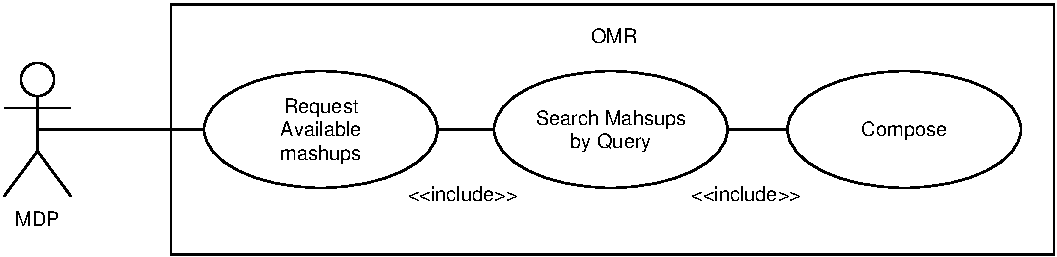
\includegraphics[width=400pt]{graphics/uc3.pdf}
\caption{Web interface use case}
\label{fig:pack-uc3}
\end{figure}
\FloatBarrier

\newpage
\subsubsection{Request available mash-ups}
\label{subsec:requestavailable}

\begin{table}[!htpb]
\centering
\begin{tabular}{|c|x{0.5cm}x{5cm}x{5cm}|}
\noalign{\hrule height 2pt}
\textbf{Use Case Name} & \multicolumn{3}{c|}{Request available mash-ups}\\
\hline
\textbf{Use Case ID} & \multicolumn{3}{x{10.5cm}|}{UC3.1}\\
\hline
\textbf{Primary Actor} & \multicolumn{3}{c|}{Web interface}\\
\hline
\textbf{Pre-Condition} & \multicolumn{3}{x{10.5cm}|}{Web interface requests dynamic  mash-up binding}\\
\hline
\textbf{Post-Condition} & \multicolumn{3}{x{10.5cm}|}{Web Interface receives a mash-up list}\\
\hline
\textbf{Flow of Events} & \multicolumn{1}{c|}{} & \multicolumn{1}{x{5cm}|}{Actor Input} & \multicolumn{1}{x{5cm}|}{System Response}\\
\hline

\textbf{} & \multicolumn{1}{x{0.5cm}|}{1a} & 
\multicolumn{1}{x{5cm}|}{Web Interface requests a service / mash-up.} & 
\multicolumn{1}{x{5cm}|}{The system provides a feed with the ranking of available  mash-ups / services.}\\
\hline

\textbf{} & \multicolumn{1}{x{0.5cm}|}{1b} & 
\multicolumn{1}{x{5cm}|}{(Optional) The system does not find a matching service / mash-up and composes a new one on the fly and returns it} & 
\multicolumn{1}{x{5cm}|}{}\\
\hline


\end{tabular}
\end{table}
\FloatBarrier

\newpage
\subsubsection{Search mash-ups by query}
\label{subsec:searchquery}

\begin{table}[!htpb]
\centering
\begin{tabular}{|c|x{0.5cm}x{5cm}x{5cm}|}
\noalign{\hrule height 2pt}
\textbf{Use Case Name} & \multicolumn{3}{c|}{Search mash-ups by query}\\
\hline
\textbf{Use Case ID} & \multicolumn{3}{x{10.5cm}|}{UC3.2}\\
\hline
\textbf{Primary Actor} & \multicolumn{3}{c|}{Web interface}\\
\hline
\textbf{Pre-Condition} & \multicolumn{3}{x{10.5cm}|}{Web interface requests dynamic  mash-up binding}\\
\hline
\textbf{Post-Condition} & \multicolumn{3}{x{10.5cm}|}{Web Interface receives a mash-up list}\\
\hline
\textbf{Flow of Events} & \multicolumn{1}{c|}{} & \multicolumn{1}{x{5cm}|}{Actor Input} & \multicolumn{1}{x{5cm}|}{System Response}\\
\hline

\textbf{} & \multicolumn{1}{x{0.5cm}|}{1a} & 
\multicolumn{1}{x{5cm}|}{Web Interface requests a service / mash-up.} & 
\multicolumn{1}{x{5cm}|}{The system provides a feed with the ranking of available  mash-ups / services.}\\
\hline

\textbf{} & \multicolumn{1}{x{0.5cm}|}{1b} & 
\multicolumn{1}{x{5cm}|}{(Optional) The system does not find a matching service / mash-up and composes a new one on the fly and returns it} & 
\multicolumn{1}{x{5cm}|}{}\\
\hline


\end{tabular}
\end{table}
\FloatBarrier


\subsection{Conclusions}

With the use cases described we have introduced the basic functionalities that have been implemented in this project. They help us to understand the different actors that can interact. They can serve as a base for further development and different use cases that can come to mind. They do not cover mash-up composition, this could be considered for future work lines.
